%%%%%%%%%%%%%%%%%%%%%%%%%%%%%%%%%%%%%%%%%
% Beamer Presentation
% LaTeX Template
% Version 1.0 (10/11/12)
%
% This template has been downloaded from:
% http://www.LaTeXTemplates.com
%
% License:
% CC BY-NC-SA 3.0 (http://creativecommons.org/licenses/by-nc-sa/3.0/)
%
%%%%%%%%%%%%%%%%%%%%%%%%%%%%%%%%%%%%%%%%%

%----------------------------------------------------------------------------------------
%	PACKAGES AND THEMES
%----------------------------------------------------------------------------------------

\documentclass{beamer}

\mode<presentation> {
	
	% The Beamer class comes with a number of default slide themes
	% which change the colors and layouts of slides. Below this is a list
	% of all the themes, uncomment each in turn to see what they look like.
	
	%\usetheme{default}
	%\usetheme{AnnArbor}
	%\usetheme{Antibes}
	%\usetheme{Bergen}
	%\usetheme{Berkeley}
	%\usetheme{Berlin}
	%\usetheme{Boadilla}
	%\usetheme{CambridgeUS}
	%\usetheme{Copenhagen}
	%\usetheme{Darmstadt}
	%\usetheme{Dresden}
	%\usetheme{Frankfurt}
	%\usetheme{Goettingen}
	%\usetheme{Hannover}
	%\usetheme{Ilmenau}
	%\usetheme{JuanLesPins}
	%\usetheme{Luebeck}
	\usetheme{Madrid}
	%\usetheme{Malmoe}
	%\usetheme{Marburg}
	%\usetheme{Montpellier}
	%\usetheme{PaloAlto}
	%\usetheme{Pittsburgh}
	%\usetheme{Rochester}
	%\usetheme{Singapore}
	%\usetheme{Szeged}
	%\usetheme{Warsaw}
	
	% As well as themes, the Beamer class has a number of color themes
	% for any slide theme. Uncomment each of these in turn to see how it
	% changes the colors of your current slide theme.
	
	%\usecolortheme{albatross}
	\usecolortheme{beaver}
	%\usecolortheme{beetle}
	%\usecolortheme{crane}
	%\usecolortheme{dolphin}
	%\usecolortheme{dove}
	%\usecolortheme{fly}
	%\usecolortheme{lily}
	%\usecolortheme{orchid}
	%\usecolortheme{rose}
	%\usecolortheme{seagull}
	%\usecolortheme{seahorse}
	%\usecolortheme{whale}
	%\usecolortheme{wolverine}
	
	%\setbeamertemplate{footline} % To remove the footer line in all slides uncomment this line
	%\setbeamertemplate{footline}[page number] % To replace the footer line in all slides with a simple slide count uncomment this line
	
	%\setbeamertemplate{navigation symbols}{} % To remove the navigation symbols from the bottom of all slides uncomment this line
}

\usepackage{graphicx} % Allows including images
\usepackage{subfigure}
\usepackage{booktabs} % Allows the use of \toprule, \midrule and \bottomrule in tables
\usepackage{bm}

%----------------------------------------------------------------------------------------
%	TITLE PAGE
%----------------------------------------------------------------------------------------

\title[MSC-LASSO]{On Model Selection Consistency of Lasso} 

\author{Ganchao Wei} 
\date{December 8, 2021}

\begin{document}
	
	\begin{frame}
		\titlepage % Print the title page as the first slide
	\end{frame}
	
	\begin{frame}
		\frametitle{Overview} % Table of contents slide, comment this block out to remove it
		\tableofcontents
	\end{frame}
	
	%--------------------------------------------------------------------
	%	PRESENTATION SLIDES
	%--------------------------------------------------------------------
	
	\section{Introduction}
	
	\begin{frame}
		\frametitle{Introduction}
		The Lasso estimates $\hat{\beta}^n$ are defined by:
		$$\hat{\beta}^n(\lambda) = argmin_{\beta}||Y_n - \bm{X}_n\beta||_2^2 + \lambda||\beta||_1$$
		However, if an irrelevant predictor is highly correlated with the predictors in the true model, Lasso may not be able to distinguish it from the true predictors, with any amount of data and any amount of regularization. For example:
		\begin{itemize}
			\item 
			For a fixed $p$ and orthogonal designs, the optimal (i.t.o. parameter estimation) Lasso doesn't give consistent model selection
			\item
			When using Lasso for knot selection in spline regression, it tend to pick up knots in close proximity to one another.
		\end{itemize}
	\end{frame}
	
	
	\begin{frame}
		\frametitle{Introduction}
		In this paper, they consider model selection consistency of the Lasso. Specifically, they focus on two problems:
		\begin{itemize}
			\item 
			Whether there exists a deterministic amount of regularization that gives consistent selection.
			\item
			Whether there exists a correct amount of regularization that selects the true model, for each random realization.
		\end{itemize}
		\vspace{\baselineskip}
		They found there exists an \textbf{Irrepresentable Condition} that is almost necessary and sufficient for both types of consistency (estimation consistency + model selection consistency)
	\end{frame}
	
	\section{Model Selection Consistency and Irrepresentable Conditions}
	
	\begin{frame}
		\frametitle{Model Selection Consistency and Irrepresentable Conditions}
		Two consistencies:
		\begin{itemize}
			\item 
			Parameter estimation consistency: $\hat{\beta}^n - \beta^n \to_p 0,$ as $n \to \infty$
			\item
			Model selection consistency: $P(\{i: \hat{\beta}^n \ne 0\} = \{i: \beta^n \ne 0\}) \to 1$, as $n \to \infty$
		\end{itemize}
		To separate 2 consistencies, define the sign consistency that doesn't assume the estimates to be estimation consistent:
		\begin{figure}
			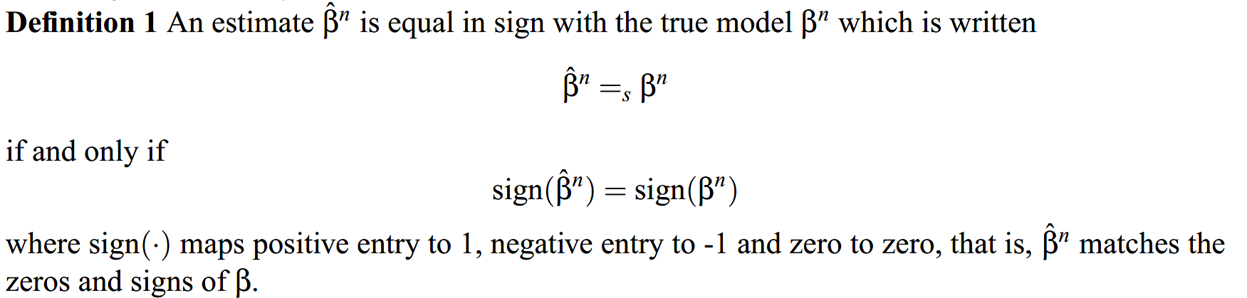
\includegraphics[width=1\linewidth]{image001.png}
		\end{figure}
	\end{frame}
	
	\begin{frame}
		\frametitle{Model Selection Consistency and Irrepresentable Conditions}
		2 sign consistencies for Lasso, depending on how the amount of regularization is determined:
		\begin{figure}
			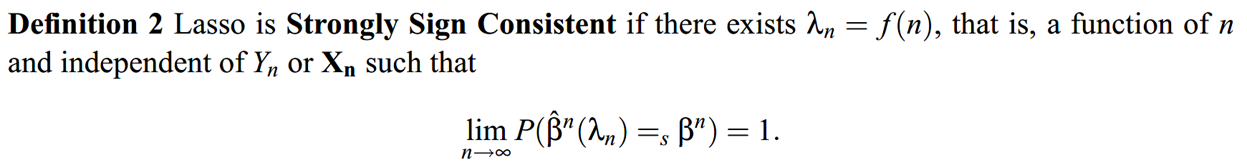
\includegraphics[width=1\linewidth]{image002.png}
			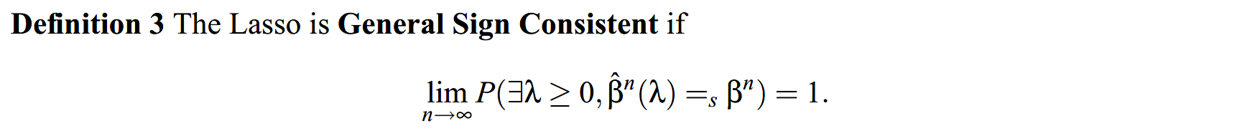
\includegraphics[width=1\linewidth]{image003.png}
		\end{figure}
		We further partition the design matrix, based on the sparsity of parameters. Then we can define the strong/ weak irrepresentable condition (next page).
		
	\end{frame}
	
	\begin{frame}
		\frametitle{Model Selection Consistency and Irrepresentable Conditions}
		\begin{figure}
			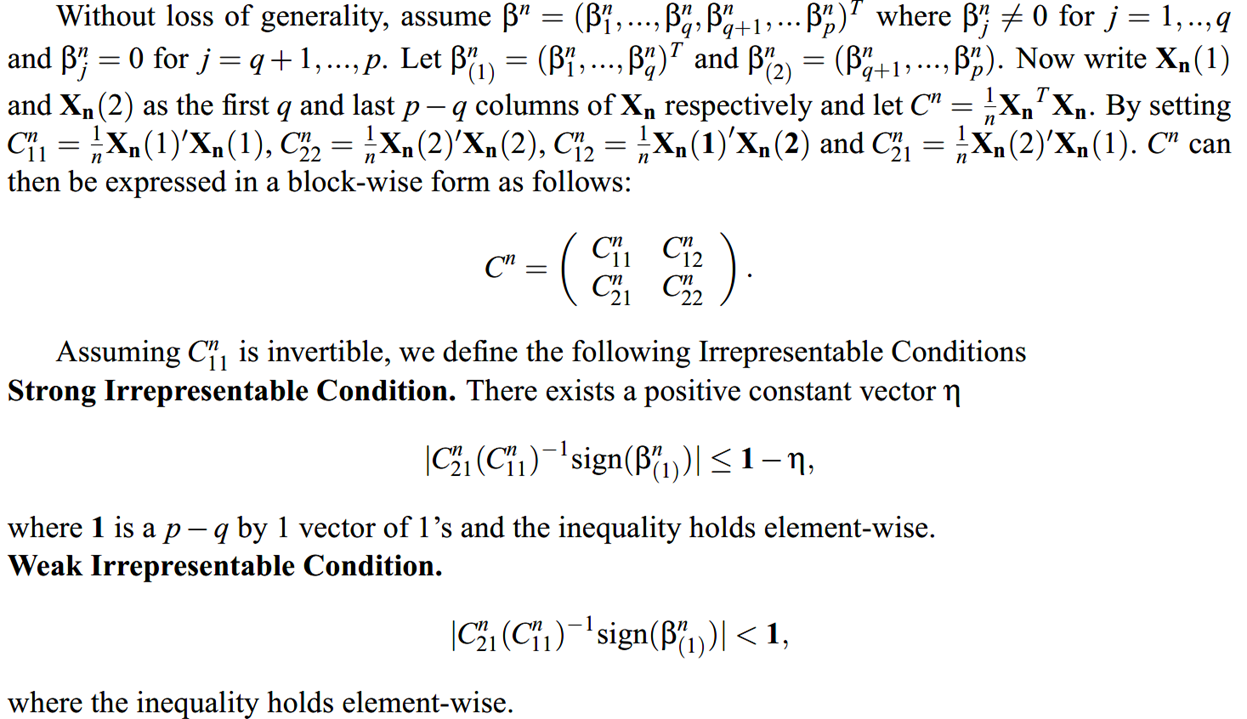
\includegraphics[width=1\linewidth]{image004.png}
		\end{figure}
	\end{frame}
	
	\begin{frame}
		\frametitle{Model Selection Consistency and Irrepresentable Conditions}
		We can put a lower bound on the probability of choosing the true model. This is quantitatively relates to:
		\begin{itemize}
			\item 
			The probability of Lasso selecting the correct model.
			\item
			How well Strong Irrepresentable Condition holds.
		\end{itemize}
		 \begin{figure}
		 	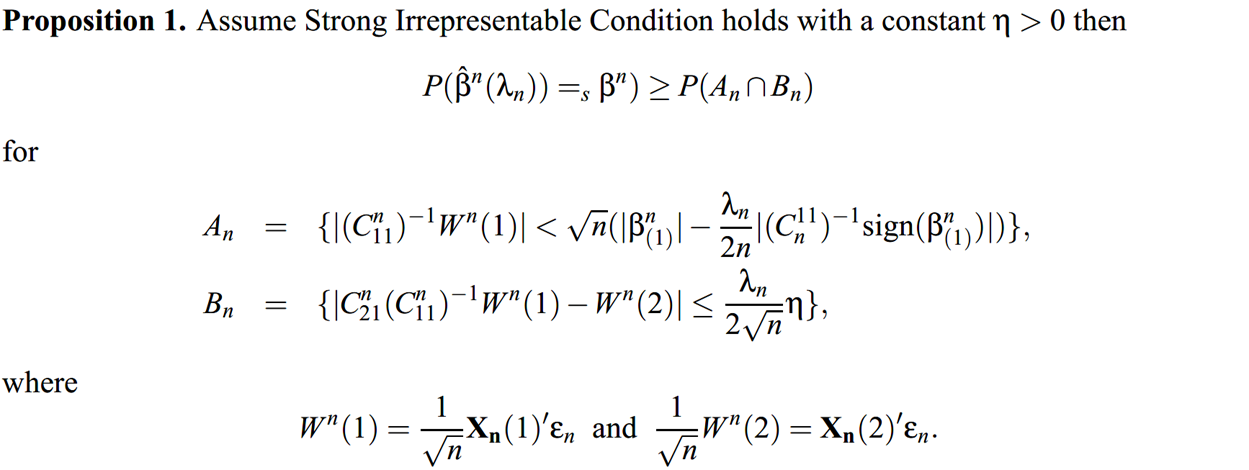
\includegraphics[width=1\linewidth]{image005.png}
		 \end{figure}
	\end{frame}
	
	\begin{frame}
		\frametitle{Model Selection Consistency and Irrepresentable Conditions}
		Some interpretations:
		\begin{itemize}
			\item 
			$A_n$: the signs of those of $\beta_{(1)}^n$ are estimated correctly.
			\item
			Given $A_n$, $B_n$ further imply $\hat{\beta}^n_{(2)}$ are shrunk to zero.
			\item
			$\lambda_n$ trades off the size of these 2 events: smaller leads to larger $A_n$ but smaller $B_n$ $\Rightarrow$ more likely to have Lasso pick more irrelevant variables.
			\item
			larger $\eta$  $\Rightarrow$ easier for Lasso to pick up true model (larger $B_n$ but not impact on $A_n$)
		\end{itemize}
	\end{frame}
	
	
	\section{Model Selection Consistency for Small $q$ and $p$}
	
	\begin{frame}
		\frametitle{Model Selection Consistency for Small $q$ and $p$}
		We first consider $q, p$ and $\beta^n$ are fixed as $n\to \infty$. As usual, the regularity conditions:
		\begin{itemize}
			\item 
			$C^n\to C$, as $n\to \infty$, where $C$ is p.d.
			\item
			$\frac{1}{n}\max_{1\leq i\leq n}((x_i^n)^Tx_i^n) \to 0$, as $n \to \infty$
		\end{itemize}
		Then,
		\begin{figure}
			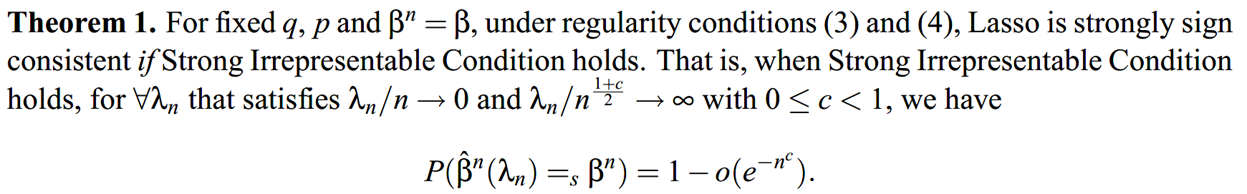
\includegraphics[width=1\linewidth]{image006.png}
		\end{figure}
	\end{frame}
	
	\begin{frame}
		\frametitle{Model Selection Consistency for Small $q$ and $p$}
		
		Theorem 1 shows: Strong Irrepresentable Condition + finite second moment of the noise $\Rightarrow$ strong sign consistency at exponentail rate\\
		\vspace{\baselineskip}
		Moreover, by Knight and Fu(2000): $\lambda_n = o(n) \Rightarrow$ LASSO has consistent estimation and asymptotic normality.\\
		\vspace{\baselineskip}
		They further show that Weak Irrepresentable Condition is also necessary for the weaker general sign consistency.
		\begin{figure}
			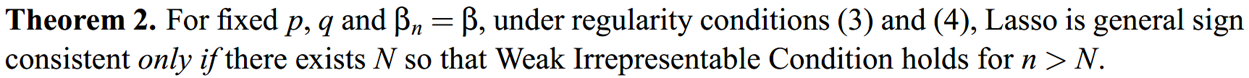
\includegraphics[width=1\linewidth]{image007.png}
		\end{figure}
	\end{frame}
	
	\section{Model Selection Consistency for Large $q$ and $p$}
	
	\begin{frame}
		\frametitle{Model Selection Consistency for Large $q$ and $p$}
		Then ,we allow the dimension of the designs $C^n$ and model parameters $\beta_n$ grow as $n$ grows (i.e. $p=p_n$ and $q = q_n$ are allowed to grow with $n$). Therefore, we need to modify the regularity conditions a bit:
		\begin{itemize}
			\item 
			$\frac{1}{n}(X_i^n)'X_i^n \leq M_1$ for $\forall i$
			\item
			Bound the eigenvalues of $C_{11}^n$: $\alpha'C_{11}^n \alpha \geq M_2$, for $\forall ||\alpha||_2^2 = 1$
			\item
			Sparsity assumption: $q_n = O(n^{c_1})$
			\item
			Control the smallest entry of $\beta_{(1)}^n$: $n^{\frac{1-c_2}{2}}\min_{i=1,\ldots,q}|\beta_i^n| \geq M_3$
		\end{itemize} 
		Then we can give the following result:
		\begin{figure}
			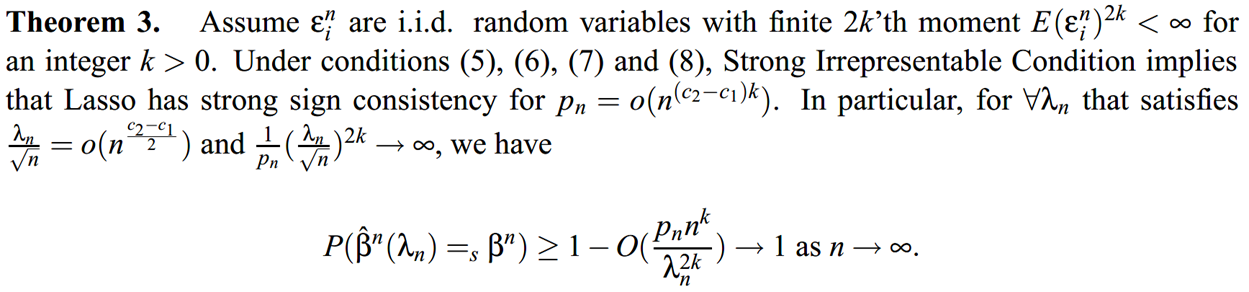
\includegraphics[width=1\linewidth]{image008.png}
		\end{figure}
	\end{frame}
		
	\begin{frame}
		\frametitle{Model Selection Consistency for Large $q$ and $p$}
		In particular, for Gaussian noise:
		\begin{figure}
			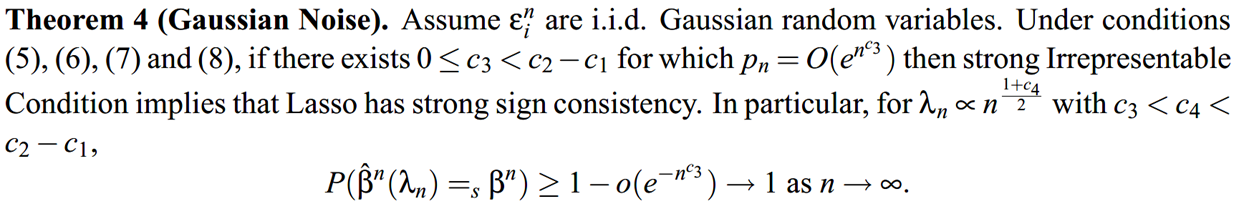
\includegraphics[width=1\linewidth]{image009.png}
		\end{figure}
	
		This is interesting: for Gaussian noise, $p$ can grow faster than $n$ (up to exponentially), while still allow for fast convergence of the probability of correct model selection to 1.\\
		\vspace{\baselineskip}
		\textbf{This is not the case for all noise distributions}.
		
	\end{frame}
	
	\section{Analysis and Sufficient Conditions for Strong Irrepresentable Condition}
	
	\begin{frame}
		\frametitle{Analysis and Sufficient Conditions for Strong Irrepresentable Condition}
		In general, the Irrepresentable Condition is non-trivial, when number of zeros and nonzeros are of moderate sizes. Therefore, they give 5 sufficient conditions, such that Strong Irrepresentable Condition is guaranteed.
		\begin{figure}
			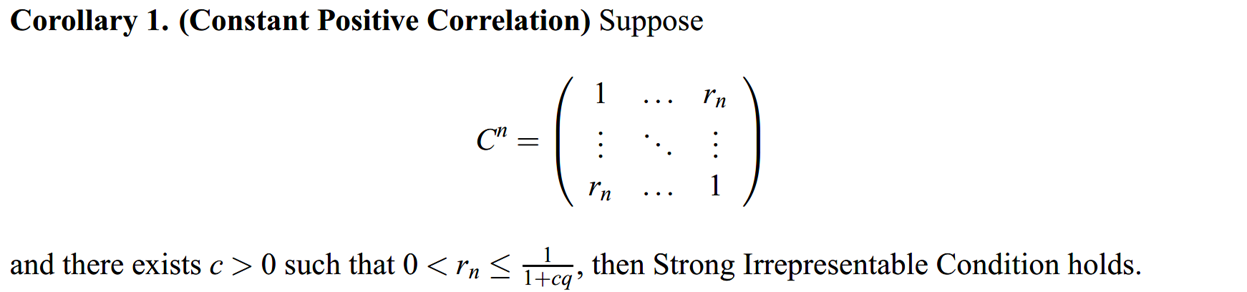
\includegraphics[width=1\linewidth]{image010.png}
		\end{figure}
		The design is symmetric, so that the covariates share a constant.
	\end{frame}
	
	\begin{frame}
		\frametitle{Analysis and Sufficient Conditions for Strong Irrepresentable Condition}
		\begin{figure}
			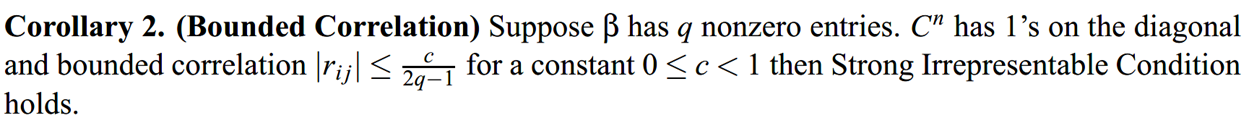
\includegraphics[width=1\linewidth]{image011.png}
		\end{figure}
		When the design matrix is slightly correlated, Lasso works consistently.
		\begin{figure}
			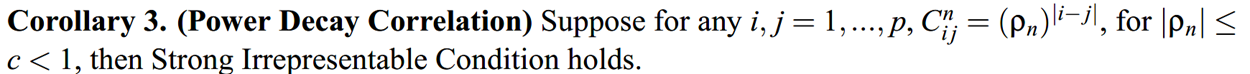
\includegraphics[width=1\linewidth]{image012.png}
			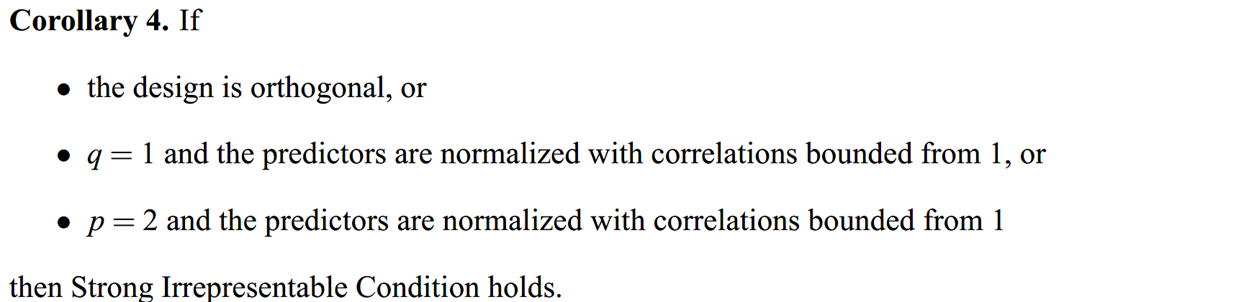
\includegraphics[width=1\linewidth]{image013.png}
		\end{figure}
	\end{frame}
	
	\begin{frame}
		\frametitle{Analysis and Sufficient Conditions for Strong Irrepresentable Condition}
		\begin{figure}
			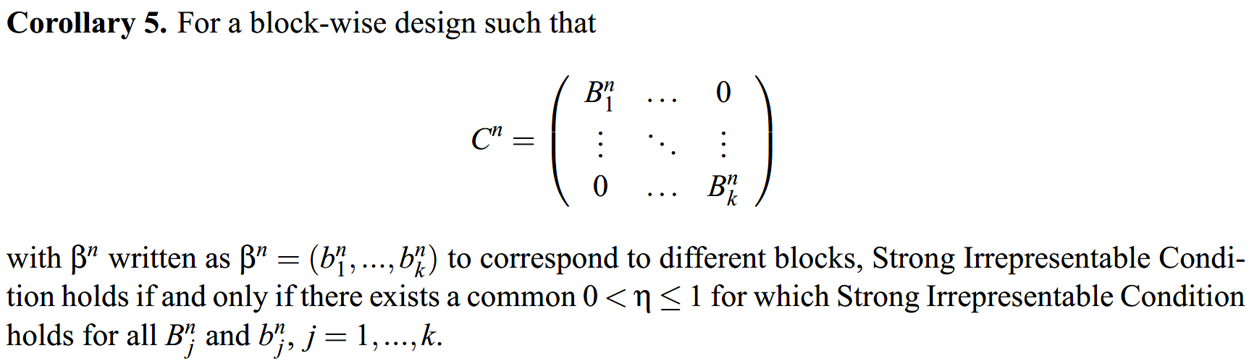
\includegraphics[width=1\linewidth]{image014.png}
		\end{figure}	
	\end{frame}
	
	\section{Simulation Studies}
	
	\begin{frame}
		\frametitle{Simulations}
		\textbf{Simulation 1}: Consistency and Inconsistency with 3 Variables\\
		Generate i.i.d. random variables $x_{i1}, x_{i2}, e_i$ and $\epsilon_i$, with variance 1 and mean 0, for $i=1,\ldots,n=1000$. $x_{i3}$ is correlated with $x_{i1}$ and $x_{i2}$:
		$$x_{i3} = \frac{2}{3}x_{i1} + \frac{2}{3}x_{i2} + \frac{1}{3}e_i$$
		The response:
		$$Y_i = x_{i1}\beta_1 + x_{i2}\beta_2 + \epsilon_i$$
		Then two settings:
		\begin{itemize}
			\item 
			Strong Irrepresentable Condition fails: $\beta_1 = 2, \beta_2 = 3$ 
			\item
			Strong Irrepresentable Condition holds: $\beta_1 = -2, \beta_2 = 3$ 
		\end{itemize}
	\end{frame}
	
	\begin{frame}
		\frametitle{Simulations}
		\textbf{Another view}:\\
		If we define $Y^*(\lambda) = Y - X\hat{\beta}(\lambda)$, then:
		\begin{figure}
			
\includegraphics[width=1.1\linewidth]{image015.png}
		\end{figure}
		If $\hat{\beta}_3 = 0$ $\Rightarrow$ signs of $X_1$'s and $X_2$'s inner products with Y agree with the signs of $\hat{\beta}_1$ and $\hat{\beta}_2$ $\Rightarrow$ For Lasso to be sign consistent, the signs of $\beta_1$ and $\beta_2$ has to disagree. ("agree to" Strong Irrepresentalbe Condition)
	\end{frame}
	
	\begin{frame}
		\frametitle{Simulations}
		\begin{figure}
			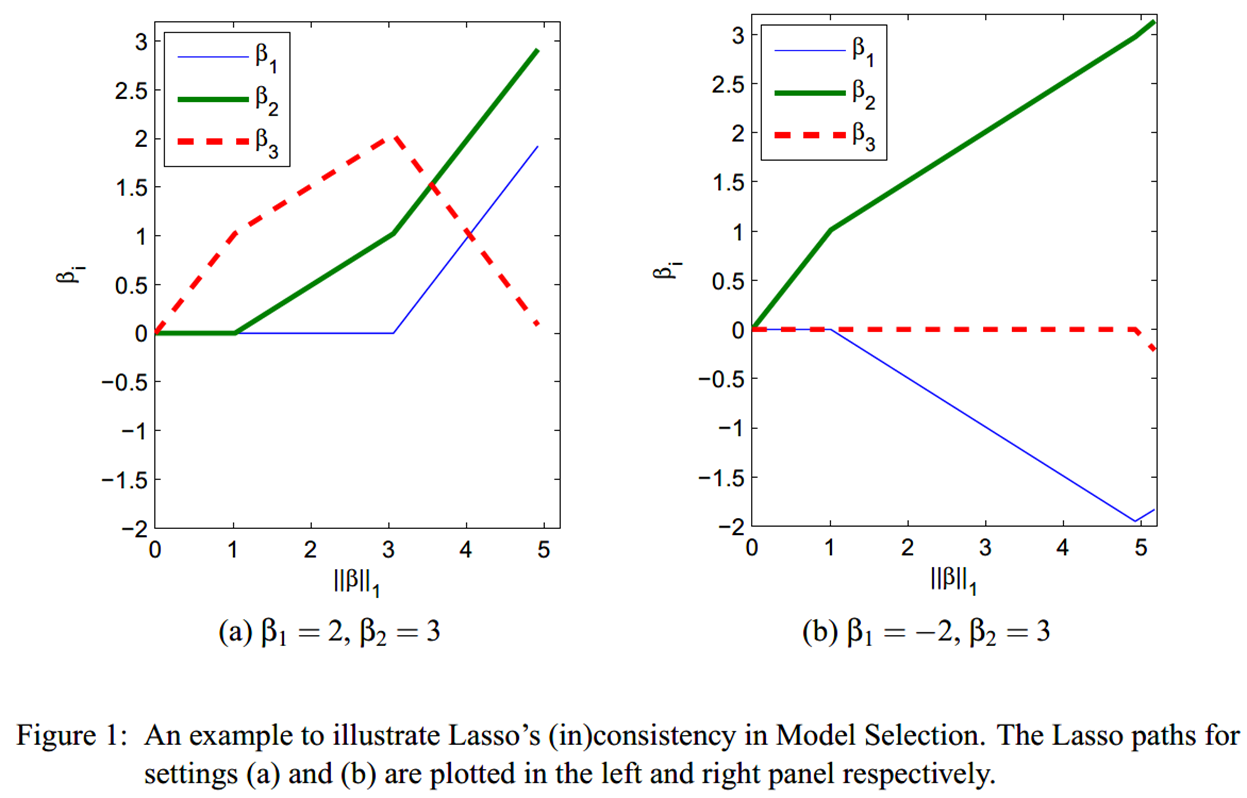
\includegraphics[width=1\linewidth]{image016.png}
		\end{figure}
	\end{frame}
	
	\begin{frame}
		\frametitle{Simulations}
		\textbf{Simulation 2}: Quantitative Evaluation of Impact of Strong Irrepresentable Condition on Model Selection\\
		Take $n=100, p = 32, q = 5, \beta_1 = (7,4,2,1,1)^T$ and choose a small $\sigma^2 = 0.1$. Calculate $\eta_{\infty} = 1 - ||C_{21}^n(C_{11}^n)^{-1}sign(\beta_{(1)}^n)||_{\infty}$.\\
		\vspace{\baselineskip}
		$\eta_{\infty} > 0$ means the Strong Irrepresentable Condition holds. The plot in the next page:
		\begin{itemize}
			\item 
			The larger $\eta_{\infty}$, the stronger the condition.
			\item
			steepest increase happens around 0.
		\end{itemize}
		
		
		 
	\end{frame}
	
	\begin{frame}
		\frametitle{Simulations}
		\begin{figure}
			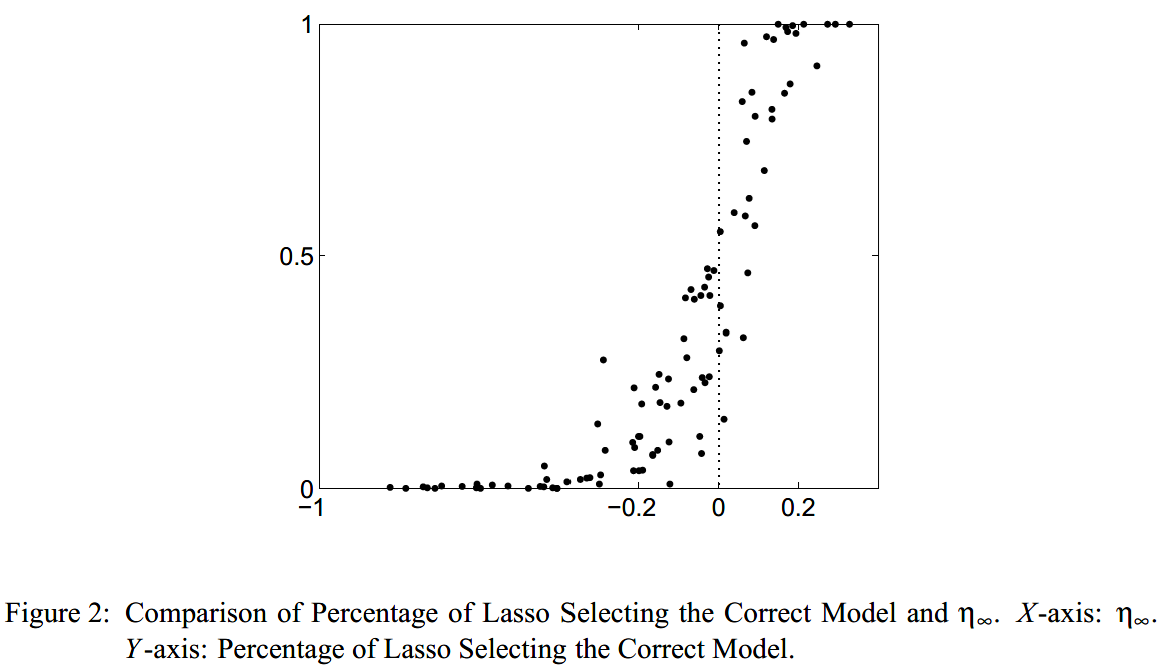
\includegraphics[width=1\linewidth]{image017.png}
		\end{figure}
	\end{frame}
	
	\begin{frame}
		\frametitle{Simulations}
		\textbf{Simulation 3}: How Strong is Irrepresentable Condition\\
		\begin{figure}
			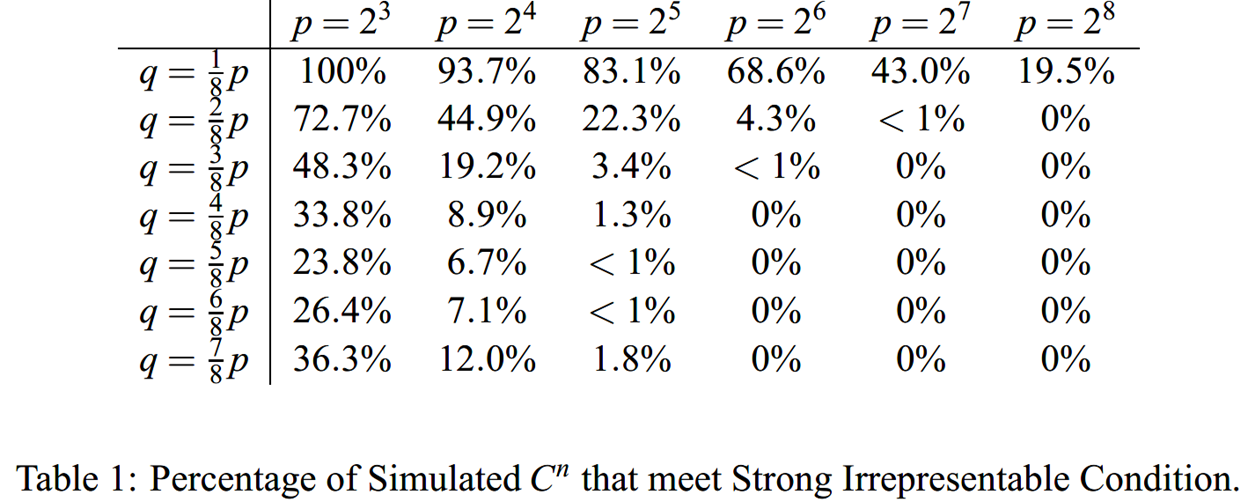
\includegraphics[width=.8\linewidth]{image018.png}
		\end{figure}
		\begin{itemize}
			\item 
			When the true model is very sparse ($q$ small), Strong Irrepresentable Condition has some probability to hold (Corollary 2)
			\item
			For the extreme case: $q=1$, it holds (Corollary 4)
			\item
			For large $p$ and $q$, the Condition rarely holds.
		\end{itemize}
	\end{frame}
	
	
\end{document}